
%(BEGIN_QUESTION)
% Copyright 2009, Tony R. Kuphaldt, released under the Creative Commons Attribution License (v 1.0)
% This means you may do almost anything with this work of mine, so long as you give me proper credit

Read selected portions of the Limitorque L120 series actuator (L120-10 through L120-40) manual published by FlowServe (document FCD LMENIM1201-01, 07/06), and answer the following questions:

\vskip 10pt

Page 24 shows an ``exploded view'' of the actuator mechanism.  Examine this illustration and identify the locations of the {\it worm gear}, {\it electric motor}, {\it limit switch assembly}, and {\it torque switch assembly}.

Note: a ``worm'' gear is a type of gear set where a screw engages with the teeth of a gear wheel to form a large speed reduction ratio:

$$\includegraphics[width=15.5cm]{i04223x01.eps}$$

\vskip 10pt

Page 18 shows an optional handwheel for the L120-40 actuator.  Examine this drawing and identify the gears used to multiply torque from the handwheel to the actuator mechanism.  Note: there are actually {\it two} sets of gears used for torque multiplication in this large handwheel: a set of {\it spur gears} and a set of {\it bevel gears}.  Identify both and try to explain their operation from the drawing.

\vskip 10pt

Page 21 shows an electrical schematic for the L120 actuators.  Identify some of the different {\it limit switches} used to detect valve position and shaft torque, and explain how they work to indicate valve status and also protect the valve and actuator from overload.

\vskip 10pt

Referencing the schematic diagram on page 21, identify the effect(s) of the purple wire failing open.

\vskip 20pt \vbox{\hrule \hbox{\strut \vrule{} {\bf Suggestions for Socratic discussion} \vrule} \hrule}

\begin{itemize}
\item{} Explain the significance of the optional jumper wire around limit switch \#8.
\item{} Explain how to interpret the ``Limit Switch Contact Development'' table shown at the bottom of the schematic page.
\item{} Explain how to interpret the Local/Off/Remote switch symbol, particularly how its switch contact positions relate to the actuator lever.
\item{} Explain why the primary winding of the control power transformer has multiple taps.
\end{itemize}

\underbar{file i04223}
%(END_QUESTION)





%(BEGIN_ANSWER)


%(END_ANSWER)





%(BEGIN_NOTES)

The worm gear (wheel) is part \#21, on the vertical shaft coupled to both the handwheel and the valve stem.  The worm screw driving this worm wheel is part \#15.  The electric motor (part \#31) sits off to the side, its shaft perpendicular to the handwheel shaft.  The geared limit switch assembly (part \#305) has a shaft perpendicular to both the electric motor and the handwheel, sensing the handwheel shaft's rotation through a bevel gear set.  The torque switch (part \#300) senses applied torque by thrust motion of the worm screw shaft (part \#15).

It is interesting to note how some of the components in this ``exploded'' view of the valve actuator are shown more than once in order to illustrate how they fit together.  A good example of this are the limit and torque switch assemblies, both shown fitting into the housing as well as engaging with their respective shafts.

\vskip 10pt

The handwheel connects to a pinion gear (part \#155), meshing with a spur gear (part \#159).  The spur gear turns a bevel pinion gear (part \#154) which meshes perpendicularly with a bevel gear (part \#153) to turn the valve shaft.  Both sets of gears act as speed reducers, multiplying torque applied at the handwheel.

\vskip 10pt

In the electrical schematic on page 21, we see a variety of switches operating at different positions of the valve's travel.  Switches \#4 and \#8 serve as valve travel limit switches, preventing the valve from traveling past certain set positions.  We also see a pair of torque switches (\#17 and \#18) in place to interrupt current to the motor contactor coils if motor torque exceeds a pre-set threshold.

\vskip 10pt

If the purple wire fails open, the valve will still open and close, but only so long as someone continues to hold the ``open'' or ``close'' pushbutton.  Without continuity through the purple wire, the actuator will not {\it latch} in either direction.  









\filbreak \vskip 20pt \vbox{\hrule \hbox{\strut \vrule{} {\bf Virtual Troubleshooting} \vrule} \hrule}

\noindent
{\bf Predicting the effect of a given fault:} present each of the following faults to the students, one at a time, having them comment on all the effects each fault would produce.

\begin{itemize}
\item{} Switch \#4 fails open
\item{} Switch \#7 fails open
\item{} Switch \#17 fails shorted
\item{} Gear mechanism jams (so motor cannot turn at all)
\item{} Jumper wire around switch \#8 left disconnected on a torque-seating valve
\item{} Jumper wire around switch \#8 in place on a limit-seating (non-torque seating) valve
\end{itemize}


\vskip 10pt


\noindent
{\bf Identifying possible/impossible faults:} present symptoms to the students and then have them determine whether or not a series of suggested faults could account for all the symptoms, explaining {\it why} or {\it why not} for each proposed fault:

\begin{itemize}
\item{} Symptom: {\it valve is fully closed and refuses to open when local ``open'' switch pressed}
\item{} Symptom: {\it 0 VAC measured between terminals 1 and 19 when local ``open'' switch pressed}
\item{} 120 VAC fuse blown
\item{} Thermal overload tripped
\item{} Torque switch \#18 open
\item{} No jumper wire connected around switch \#8 
\item{} Switch placed in ``Local'' position
\item{} Switch placed in ``Off'' position
\item{} Switch placed in ``Remote'' position
\item{} Pot wiper failed open (lost contact with resistive strip)
\end{itemize}


\vskip 10pt


\noindent
{\bf Determining the utility of given diagnostic tests:} present symptoms to the students and then propose the following diagnostic tests one by one.  Students rate the value of each test, determining whether or not it would give useful information (i.e. tell us something we don't already know).  Students determine what different results for each test would indicate about the fault, if anything:

\begin{itemize}
\item{} Symptom: {\it valve is fully open and refuses to close when local ``close'' switch pressed}
\item{} Symptom: {\it 18 VAC measured between two blue wires at transformer secondary}
\item{} Measure AC voltage between L1 and L3 -- {\bf No}
\item{} Measure AC voltage across electric heater terminals  -- {\bf Yes}
\item{} Observe red and green indicator lights -- {\bf Yes}
\item{} Jumper between purple wire and terminal \#1 in ``local'' mode -- {\bf No}
\item{} Jumper across switch \#1 terminals and try closing again -- {\bf Yes}
\item{} Switch to ``Remote'' mode and try closing from remote ``close'' pushbutton -- {\bf Yes}
\item{} Measure AC voltage between yellow wires on transformer secondary -- {\bf No}
\item{} Measure AC voltage across ``Stop'' switch while pressing it and local ``close'' switch simultaneously -- {\bf No}
\end{itemize}


\vskip 10pt


\noindent
{\bf Diagnosing a fault based on given symptoms:} imagine the ??? fails ??? in this system (don't reveal the fault to students!).  Present the operator's observation(s) to the students, have them consider possible faults and diagnostic strategies, and then tell them the results of tests they propose based on the following symptoms, until they have properly identified the nature and location of the fault:

\begin{itemize}
\item{} {\it }
\item{} 
\item{} 
\end{itemize}

%INDEX% Reading assignment: Limitorque L120 electric valve actuator manual

%(END_NOTES)


